% Problem 3/5 solution
\noindent
\underline{Solution:}\\

\noindent
a) XeF is not a homonuclear diatomic molecule. Thus the atomic orbitals 
that form MOs originate from different principal quantum number levels.
The MO diagram is:\\
\newpage
\noindent
\begin{figure}[h]
\centering
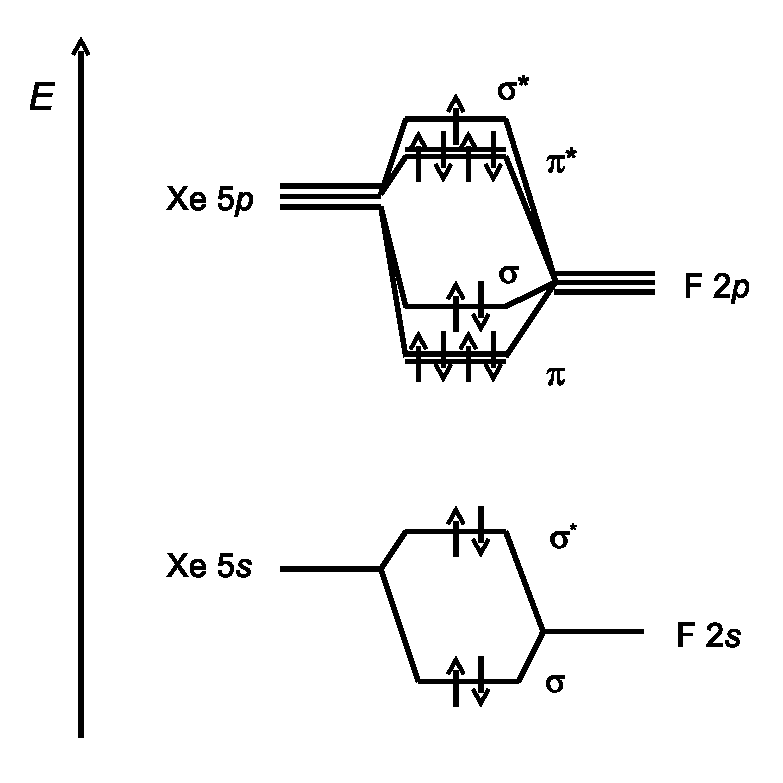
\includegraphics[scale=0.5]{xefmo}
\end{figure}

\noindent
The bond order for XeF is $(8 - 7) / 2 = 0.5$ and for XeF$^+$ $(8 - 6)
/ 2 = 1$. Thus the equilibrium bond length for XeF$^+$ is expected to be
shorter than for XeF.\\

\noindent
b) Consider the MOs of the C=C fragment:
\noindent
\begin{figure}[h]
\centering
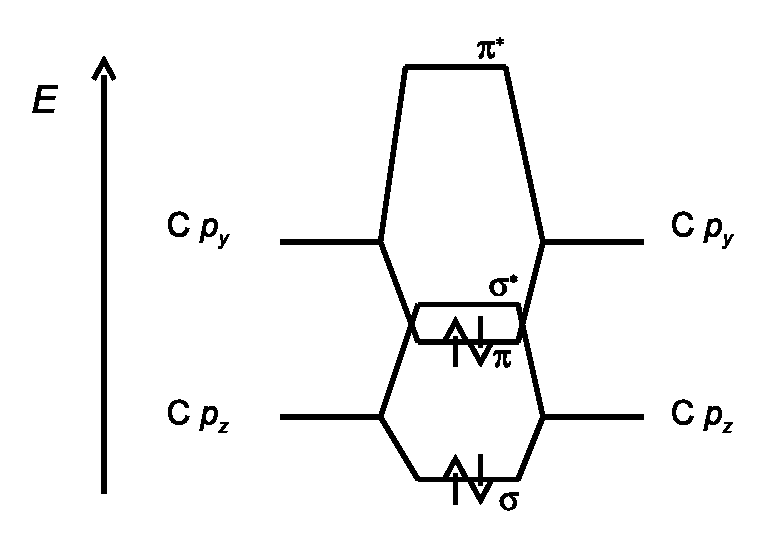
\includegraphics[scale=0.5]{ccmo}
\end{figure}

\noindent
Note that the order of the $\pi$ and $\sigma^*$ orbitals must be as shown
above. If this was not the case, the C=C fragment would not be bound!\\

\noindent
c) All the resulting bonding and antibonding orbitals become fully occupied. 
As antibonding orbitals cause more repulsion than bonding orbitals binding,
the result is no chemical binding. In general, the octet electronic
structure in atoms (e.g. rare gases) tends to lead to efficient population of the antibonding
molecular orbitals and hence they are chemically inert.\\

\hrule\vspace{0.5cm}
